\section{Kontrola kolize}\label{sec:kolize}

%Rozbor případů, kdy může nastat mezi agenty kolize (základ v MAPF).
%Rozšíření problému na agenty s nenulovou velikostí.
%Popis pomocných datových struktur.

Při~hledání cest musí algoritmus brát v~potaz již naplánované agenty.
Pro~tyto účely jsem si vytvořil následující pomocnou datovou strukturu, do~které ukládám potřebné informace.

\paragraph{Tabulka~obsazených~pozic}\label{par:obsazene_pozice} si pamatuje pro~každý krok množinu dvojic vrcholu a agenta.
Díky této struktuře můžu jednoduše a rychle zjistit,
zda~se v~daný krok vyskytuje již naplánovaný agent na~určeném vrcholu, a popřípadě o~kterého agenta se~jedná.
Po~každém naplánování agenta je postupně přidána dvojice do~každého kroku, kdy~se agent vyskytuje na~křižovatce,
aby byla \nameref{par:obsazene_pozice} aktuální.
Tento postup přidávání agenta shrnu do funkce
\textrm{add\_planned\_agent(step, agent)}\labeltext{\textrm{add\_planned\_agent}}{str:kol_add_planned_agent}.

Kontrola kolize probíhá třemi fázemi, kontroluje se~\nameref{subsec:bezpecnost_vrcholu},
\nameref{subsec:cesta_do_vrcholu} a \nameref{subsec:cesta_z_vrcholu}.

\paragraph{Safe distance}\label{par:safe_distance} (značený~$d$) určuje minimální povolenou vzdálenost mezi dvěma agenty.
\nameref{par:safe_distance} je společný parametr všech kontrol a lze nastavit před~spuštěním simulace.
Nenulová hodnota \nameref{par:safe_distance} má šanci snížit kolize,
pokud jsou zavedené nepřesnosti parametrem \nameref{par:odchylka}.

Jelikož se můžou agenti v~libovolný okamžik jakkoliv natočit, pracuji ve~výpočtech se zjednodušeným modelem agentů.
Namísto počítání složitého aktuálního natočení agenta a následné převedení na~obdélník,
je agent nahrazen pomyslným kruhem.

\paragraph{Poloměr agenta}\label{par:polomer_agenta} určuje poloměr kruhu zjednodušeného modelu
a spočítá se z~agentovo délky~$l$ a šířky~$w$ jako $\frac{\sqrt {l^2 + w^2}}{2}$.
Kontroly poté zjišťují, jestli jsou kruhy tvořené pozicí agenta a jeho poloměrem disjunktní.
Jinými slovy agenti jsou kontrolami vyhodnoceni v~kolizních trasách,
pokud se během cesty středy agentů přiblíží na~vzdálenost menší nebo rovnu součtu jejich poloměrů a \emph{safe distance}.
Toto zjednodušení nemůže způsobit kolizi, jelikož je celý agent umístěn uvnitř \hyperref[par:polomer_agenta]{poloměru agenta}.
Zároveň počítání s~kruhem značně zrychluje samotný výpočet.

\subsection{Bezpečnost vrcholu}\label{subsec:bezpecnost_vrcholu}

%Popis postupu kontroly, pseudokód, náčrtek.

\hyperref[subsec:bezpecnost_vrcholu]{Kontrola bezpečnosti vrcholu} zjišťuje,
zda~je bezpečný výskyt agenta v~určitém kroku na~určeném vrcholu.
Kontrola je rozšíření první \ref{str:mapf} podmínky
\uv{žádní dva agenti se nesmí nacházet na~stejném vrcholu v~jednom kroku} \eqref{eq:mapf_kolize_vrchol}.

Tato kontrola pracuje s~vrcholem~$v$, krokem~$s$ a poloměrem agenta~$r$, pro~kterého je kontrola určená.
Dále algoritmus zná maximální povolenou velikost agenta.
Z~maximální délky a šířky je předpočítán maximální poloměr agenta~$m$.

Na~obrázku (Obrázek~\ref{fig:kolize_na_vrcholu}) je ukázka situací, které tato kontrola vyhodnotí jako kolizní.
Vlevo dochází ke~kolizi, jelikož jsou dva agenti na~stejném vrcholu.
Vpravo nastává situace, kdy~jsou dva vrcholy a agenti na~nich příliš blízko.
Situace je kontrolou vyhodnocena jako kolizní i~když se agenti nepřekrývají.

\begin{figure}[h]
	\centering
	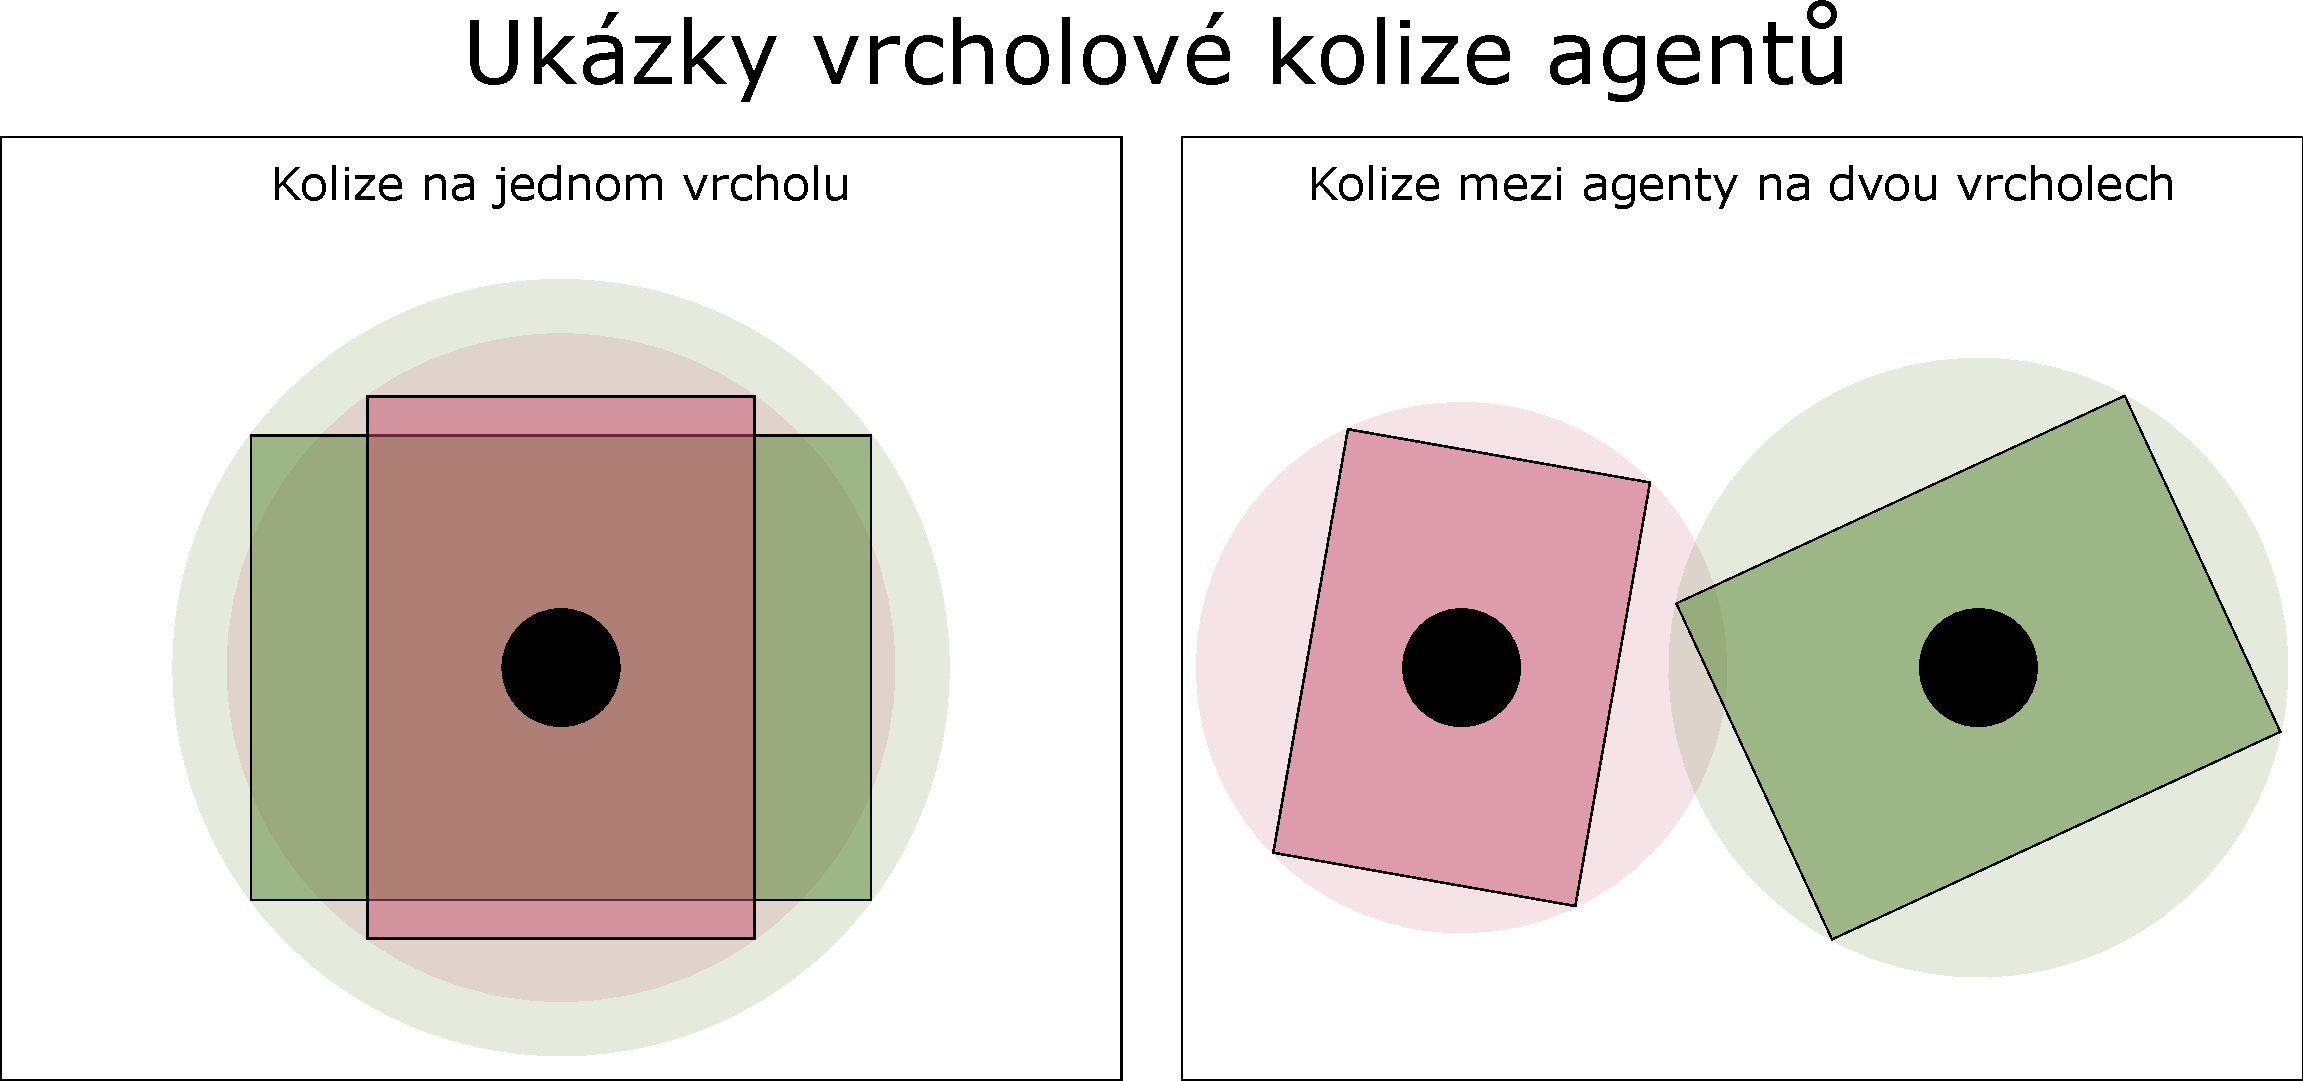
\includegraphics[width=\textwidth]{../img/kolize_vrchol}
	\caption{
		Ukázka kolizních situací, které jsou detekovány \hyperref[subsec:bezpecnost_vrcholu]{kontrolou bezpečnosti vrcholu}.
		Na~obrázcích jsou černě zobrazeny vrcholy.
		Obdélníky reprezentují agenty a kruhy tvoří bezpečnou zónu příslušných agentů.
	}
	\label{fig:kolize_na_vrcholu}
\end{figure}

Kontrola pro~vrchol $v$ začne procházet všechny vrcholy grafu od~nejbližšího $v$ podle eukleidovské vzdálenosti.
Pro~každý vrchol~$u$, který je blíže než~$r + d + m$, se nejprve zjistí,
jestli je na~vrcholu~$u$ v~kroku~$s$ nějaký agent.
Pokud není, pokračuje kontrola dalším vrcholem.
Jinak se spočítá poloměr agenta~$r'$ nacházejícího se v~kroku~$s$ na~vrcholu~$u$.
Pokud je eukleidovská vzdálenost vrcholů $u$ a $v$ menší nebo rovna~$r + r' + d$, kontrola selže.
V~opačném případě přejde kontrola na~další vrchol.
Pro~vrcholy vzdálené více než~$r + d + m$ uspěje kontrola triviálně,
neexistuje možnost že by agenti na~těchto vrcholech byly v~kolizi.

Níže je popsaný algoritmus na~kontrolu bezpečnosti vrcholu.

\labeltext{\textrm{safe\_vertex}}{alg:kol_safe_vertex}
% @formatter:off
\begin{code}[fontsize=\footnotesize]
// konstanty tabulka obsazených pozic t, minimální vzdálenost agentů d,
// maximální poloměr agenta m

// vstup krok, vrchol, poloměr agenta
// výstup true pokud může agent být na v, jinak false
safe_vertex(s, v, r)
  for u in sorted(V, x -> dist(x, v))
    if dist(u, v) > r + m + d
      return true
    else
      n <- t[s][v]
      r' <- diameter(n)
      if dist(u, v) <= r + r' + d
        return false
return true
\end{code}
% @formatter:on

\subsection{Cesta do~vrcholu}\label{subsec:cesta_do_vrcholu}

%Popis postupu kontroly, pseudokód, náčrtek.

\hyperref[subsec:cesta_do_vrcholu]{Kontrola cesty do~vrcholu} zjišťuje,
zda~může plánovaný agent bezpečně přejet do~určeného vrcholu v~určitém kroku,
aniž by došlo ke~kolizi s~nějakým agentem opouštějícím daný vrchol.
Kontrola zahrnuje druhou \ref{str:mapf} podmínku
\uv{žádní dva agenti nesmí projíždět stejnou hranou v~jednom kroku} \eqref{eq:mapf_kolize_hrana}.
Avšak jelikož mají agenti nenulovou velikost, je nutné kontrolovat i~případy, kdy agenti neprojíždí stejnou hranou.
Tyto situace jsou častější čím menší úhel je mezi sousedy vrcholu.
Například pro~čtvercový typ, kde je úhel mezi sousedy $90^\circ$, nastává tato kolize pouze pro~velké agenty.
U~oktagonálního typu křižovatky dochází ke~kolizi mnohem častěji, protože úhel mezi sousedy činí $45^\circ$.
Ukázka kolizního stavu je zobrazena na~obrázku (Obrázek~\ref{fig:kolize_cesta_do}).

\begin{figure}[h]
	\centering
	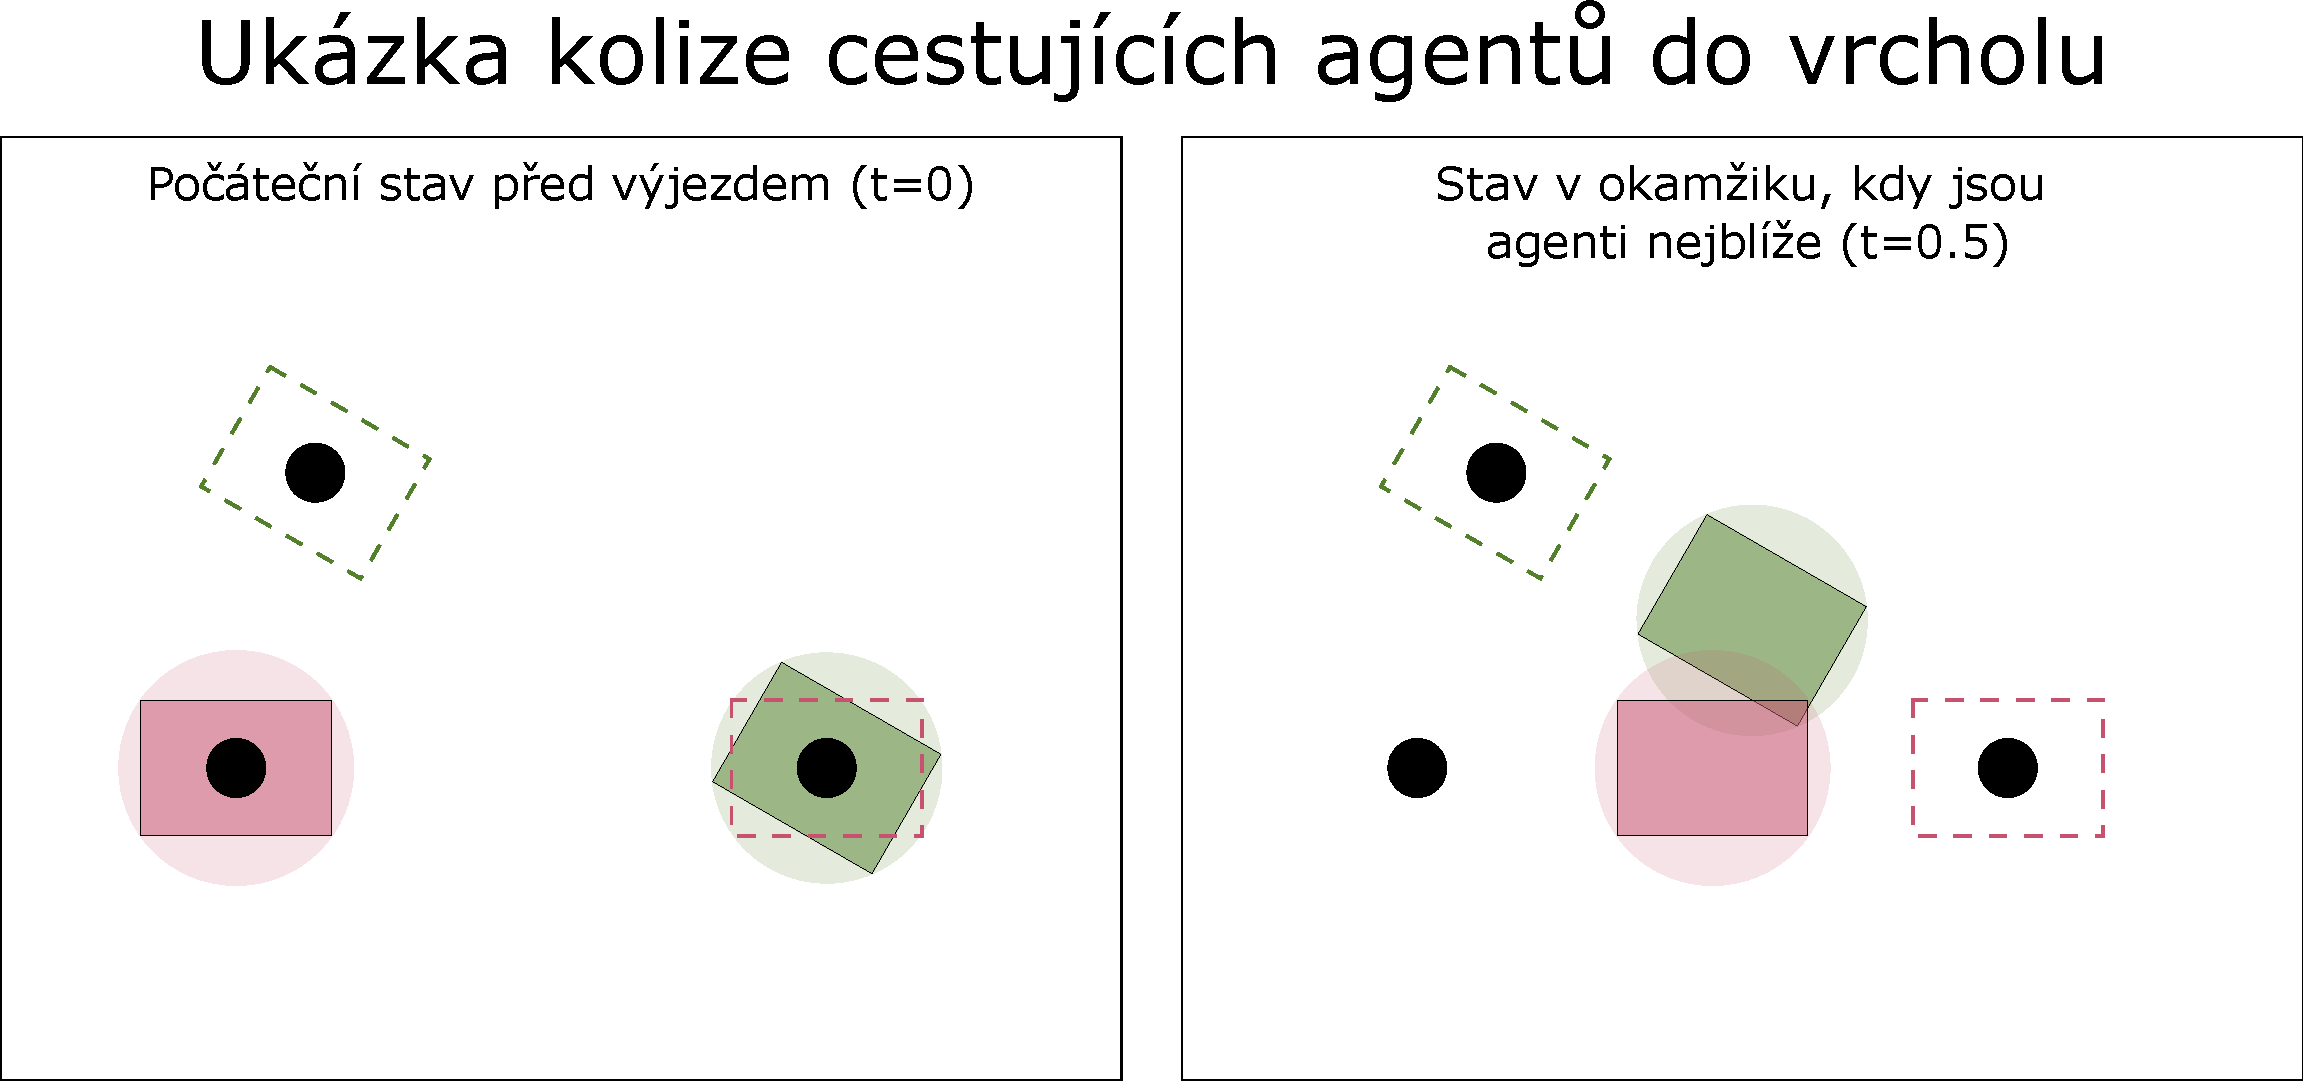
\includegraphics[width=\textwidth]{../img/kolize_cesta_do}
	\caption{
		Ukázka kolizní situace, která je detekována \hyperref[subsec:cesta_do_vrcholu]{kontrolou cesty do~vrcholu}.
		Na~obrázcích jsou černě zobrazeny vrcholy.
		Obdélníky reprezentují agenty a kruhy tvoří bezpečnou zónu příslušných agentů.
		Čárkované prázdné obdélníky značí cílové stavy agentů po~jednom kroku.
		Zelený agent je již naplánovaný, černevý je aktuálně plánován.
	}
	\label{fig:kolize_cesta_do}
\end{figure}


Tato~kontrola probíhá, pokud agent~$a$ opouští vrchol~$u$ v~kroku~$s$ a přijíždí do~vrcholu~$v$ v~následujícím kroku~$s + 1$.
Algoritmus nejprve zjistí, zda existuje naplánovaný agent~$b$, který je v~kroku~$s$ na~$v$.
Pokud žádný takový agent neexistuje, kontrola uspěje a agetova cesta z~$u$ do~$v$ v~kroku $s$ je bezpečná.
Jinak se zjistí vrchol~$w$, na~kterém se nachází agent~$b$ v~následujícím kroku $s + 1$.
Pokud nastane speciální případ $u=w$, odpovídá stav zmiňované \ref{str:mapf} podmínce \eqref{eq:mapf_kolize_hrana}.

Jelikož kontrola zná pozice vrcholů $u$, $v$ a $w$, je schopna dopočítat si čas, ve~kterém se agenti nejvíce přiblíží.
Pokud se agenti srazí, musí být v~kolizní poloze i~v~čase, kdy~jsou sobě nejblíže.
Naopak pokud jsou dostatečně daleko i~když jsou si nejblíže, při~cestě nemůže dojít ke~kolizi.
Proto stačí zkontrolovat vzdálenost v~čase, kdy~jsou agenti nejblíž.

Označím polohu agenta~$a$ jako $[x_a, y_a]$ a polohu agenta~$b$ jako $[x_b, y_b]$.
Stejným způsobem si označím pozice vrcholů $u$, $v$ a $w$ jako $[x_u, y_u]$, $[x_v, y_v]$ resp. $[x_w, y_w]$.
Dále si označím čas mezi kroky~$s$ a $s + 1$ jako~$t\in[0, 1]$.
Pro~$t = 0$ je poloha agenta~$a$ shodná s~pozicí vrcholu~$u$ a poloha agenta~$b$ shodná s~pozicí vrcholu~$v$.
Analogicky v~čase $t = 1$ se nachází agent~$a$ na~vrcholu~$v$ a agent~$b$ na~vrcholu~$w$.

Jelikož se agenti pohybují po~úsečce mezi vrcholy,
pro~$t\in[0, 1]$ se agent $a$ nachází na~$x_a = tx_u + (1 - t)x_v$, $y_a = ty_u + (1 - t)y_v$.
Poloha agenta~$b$ je analogicky $x_b = tx_v + (1 - t)x_w$ a $y_b = ty_v + (1 - t)y_w$.
Vzdálenost agentů v~závislosti na~čase~$t$ je $\sqrt{(x_a - x_b)^2 + (y_a - y_b)^2}$.
Dále upravím vzorec pod~odmocninou.
\begin{align*}
	((x_a - x_b)^2 &+ (y_a - y_b)^2) = \\
	((tx_u + (1 - t)x_v - tx_v - (1 - t)x_w)^2 &+ (ty_u + (1 - t)y_v - ty_v - (1 - t)y_w)^2) = \\
	((tx_u + x_v - tx_v - tx_v - x_w + tx_w)^2 &+ (ty_u + y_v - ty_v - ty_v - y_w + ty_w)^2) = \\
	((t(x_u - x_v - x_v + x_w) + x_v - x_w)^2 &+ (t(y_u - y_v - y_v + y_w) + y_v - y_w)^2) = \\
	(t(x_u - x_v - x_v + x_w) + x_v - x_w)^2 &+ (t(y_u - y_v - y_v + y_w) + y_v - y_w)^2 = \\
	(t(x_u - 2x_v + x_w) + x_v - x_w)^2 &+ (t(y_u - 2y_v + y_w) + y_v - y_w)^2 \\
\end{align*}

Pro~zjednodušení si označím
\begin{align*}
	x_0 &= x_u - 2x_v + x_w &\qquad
	x_1 &= x_w - x_v \\
	y_0 &= y_u - 2y_v + y_w &\qquad
	y_1 &= y_w - y_v
\end{align*}

Dosazením do~předchozího vzorce dostávám
\begin{align*}
	((x_a - x_b)^2 &+ (y_a - y_b)^2) = \\
	(t(x_u - 2x_v + x_w) + x_v - x_w)^2 &+ (t(y_u - 2y_v + y_w) + y_v - y_w)^2 = \\
	(tx_0 - x_1)^2 &+ (ty_0 - y_1)^2
\end{align*}

Pro~nalezení nejmenší vzdálenosti zjistím čas~$t$, ve~kterém se agenti nacházejí nejblíže.
K~tomu spočítám derivaci vzdálenosti a zjistím, kdy je rovna nule.
Nejprve využiji faktu, že $\min\left(\sqrt{x}\right) = \min(x) \Rightarrow \frac{d}{dx} \sqrt {x} = 0 \leftrightarrow \frac{d}{dx} x=0$.
Následně
\begin{align}
	\frac{d}{dt} \sqrt{(x_a - x_b)^2 + (y_a - y_b)^2} &= 0 \nonumber \\
	\frac{d}{dt} ((x_a - x_b)^2 + (y_a - y_b)^2) &= 0 \nonumber \\
	\frac{d}{dt} ((tx_0 - x_1)^2 + (ty_0 - y_1)^2) &= 0 \nonumber \\
	\frac{d}{dt} (tx_0 - x_1)^2 + \frac{d}{dt} (ty_0 - y_1)^2 &= 0 \nonumber \\
	2(tx_0 - x_1)x_0 + 2(ty_0 - y_1)y_0 &= 0 \nonumber \\
	tx_0^2 - x_0 x_1 + ty_0 - y_0 y_1 &= 0 \nonumber \\
	t(x_0^2 + y_0^2) &= x_0 x_1 + y_0 + y_1 \label{eq:kol_d_dt}
\end{align}

Rozeberu dva případy podle podmínky
\begin{gather}
	x_0^2 + y_0^2 = 0\label{kol:nulova_podminka}
\end{gather}

Pokud je splněna podmínka~\ref{kol:nulova_podminka}, platí $x_0^2 = 0$ a $y_0^2 = 0$.
Odtud
\begin{align*}
	x_u - 2 x_v + x_w &= 0 \\
	x_u + x_w &= 2 x_v \\
	\frac{x_u + x_w}{2} &= x_v
\end{align*}
Předchozí rovnosti jsou splněné pouze když se~$x_v$ nachází přesně uprostřed $x_u$ a $x_w$.
Analogicky $y_0^2 = 0 \Leftrightarrow \frac{y_u + y_w}{2} = y_v$, tedy $y_v$ je přesně uprostřed $y_u$ a $y_w$.
Obě tyto podmínky jsou splněny jenom když se vrchol~$v$ nachází uprostřed úsečky z~$u$ do~$w$.

V~tom případě se agenti nepovoleně přiblíží pokud vzdálenost vrcholů $v$ a $w$ je menší než
součet poloměru agentů $d_a$ a $d_b$ a dovolené vzdálenosti mezi~agenty \hyperref[par:safe_distance]{safe distance}~$d$.
Dostávám tedy nerovnost $(x_w - x_v)^2 + (y_w - y_v)^2 = x_1^2 + y_1^2 > (d_a + d_b + d)^2$.


Pokud podmínka~\ref{kol:nulova_podminka} neplatí, je možné spočítat čas~$t'$,
kdy~jsou agenti nejblíže vyjádřením z~\ref{eq:kol_d_dt}.
\begin{equation}
	\label{eq:kol_t}
	t' = \frac{x_0 x_1 + y_0 y_1}{x_0^2 + y_0^2}
\end{equation}

Po~dopočítání času spočítám vzdálenost agentů $a$ a $b$ v~čase~$t'$.
Rozdíl $x$-ové souřadnice agentů je roven
\begin{gather*}
	t' x_u + (1 - t')x_v - (t' x_v + (1 - t')x_w) =
	t' x_u + x_v - t' x_v - t' x_v - x_w + t' x_w = \\
	t'(x_u - 2x_v + x_w) + x_v - x_w =
	t' x_0 - x_1
\end{gather*}

Obdobně rozdíl $y$-ové souřadnice činí $t' y_0 - y_1$.
Pro~tento případ kontrola projde jenom pokud $(t' x_0 - x_1)^2 + (t' y_0 - y_1)^2 > (r_a + r_b + d)^2$.

Pro~výsledný algoritmus si nejdříve nadefinuji
pomocnou funkci \textrm{safe\_neighbour}\labeltext{\textrm{safe\_neighbour}}{str:safe_neighbour}.
Tato~funkce pomocí postupu výše zkontroluje, zda-li dojde ke~kolizi mezi agenty $a$ a $b$,
pokud už~známe vrcholy $u$, $v$ a $w$.

\labeltext{\textrm{safe\_neighbour}}{alg:kol_safe_neighbour}
% @formatter:off
\begin{code}[fontsize=\footnotesize]
// konstanty bezpečná vzdálenost d

// agent a s poloměrem da cestuje z u do v,
// agent b s poloměrem db cestuje z v do w
safe_neighbour(v, u, w, da, db)
  if u is w
    return false

  x0 <- u.x - 2*v.x + w.x
  x1 <- w.x - v.x
  y0 <- y.u - 2*v.y + w.y
  y1 <- w.y - v.y

  // vzdálenost mezi středy agentů na druhou
  dist <- (da + db + d) ** 2

  if x0 is 0 and y0 is 0
    return x1 ** 2 + y1 ** 2 > dist
  else
    t' <- (x0 * x1 + y0 * y1 ) / (x0 ** 2 + y0 ** 2)
    x_diff <- (t' * x0 - x1) ** 2
    y_diff <- (t' * y0 - y1) ** 2
    return x_diff + y_diff > dist
\end{code}
\label{alg:check_neighbour}
% @formatter:on

Výsledný algoritmus kolize vypadá následovně.

\labeltext{\textrm{safe\_step\_to}}{alg:kol_safe_step_to}
% @formatter:off
\begin{code}[fontsize=\footnotesize]
// konstanty tabulka obsazených pozic t

// agent a s poloměrem da cestuje z vrcholu u do v v kroku s
safe_step_to(s, u, v, da)
  b <- t[s][v]
  if b is NULL
    return true

  w <- b.path[s + 1]
  db <- diameter(b)
  return safe_neighbour(v, u, w, da, db)
\end{code}
% @formatter:on

\subsection{Cesta z~vrcholu}\label{subsec:cesta_z_vrcholu}

%Popis postupu kontroly, pseudokód.


Poslední kontrola ověřuje opačný případ předchozí kontroly.
Zjišťuje se, zda plánovaný agent~$a$ může bezpečně odjet z~vrcholu~$v$
aniž by~se srazil s~jiným již naplánovaným agentem~$b$ cestujícím do~$v$.
Ukázka kolizního stavu je zobrazena na~obrázku (Obrázek~\ref{fig:kolize_cesta_z}).

\begin{figure}[h]
	\centering
	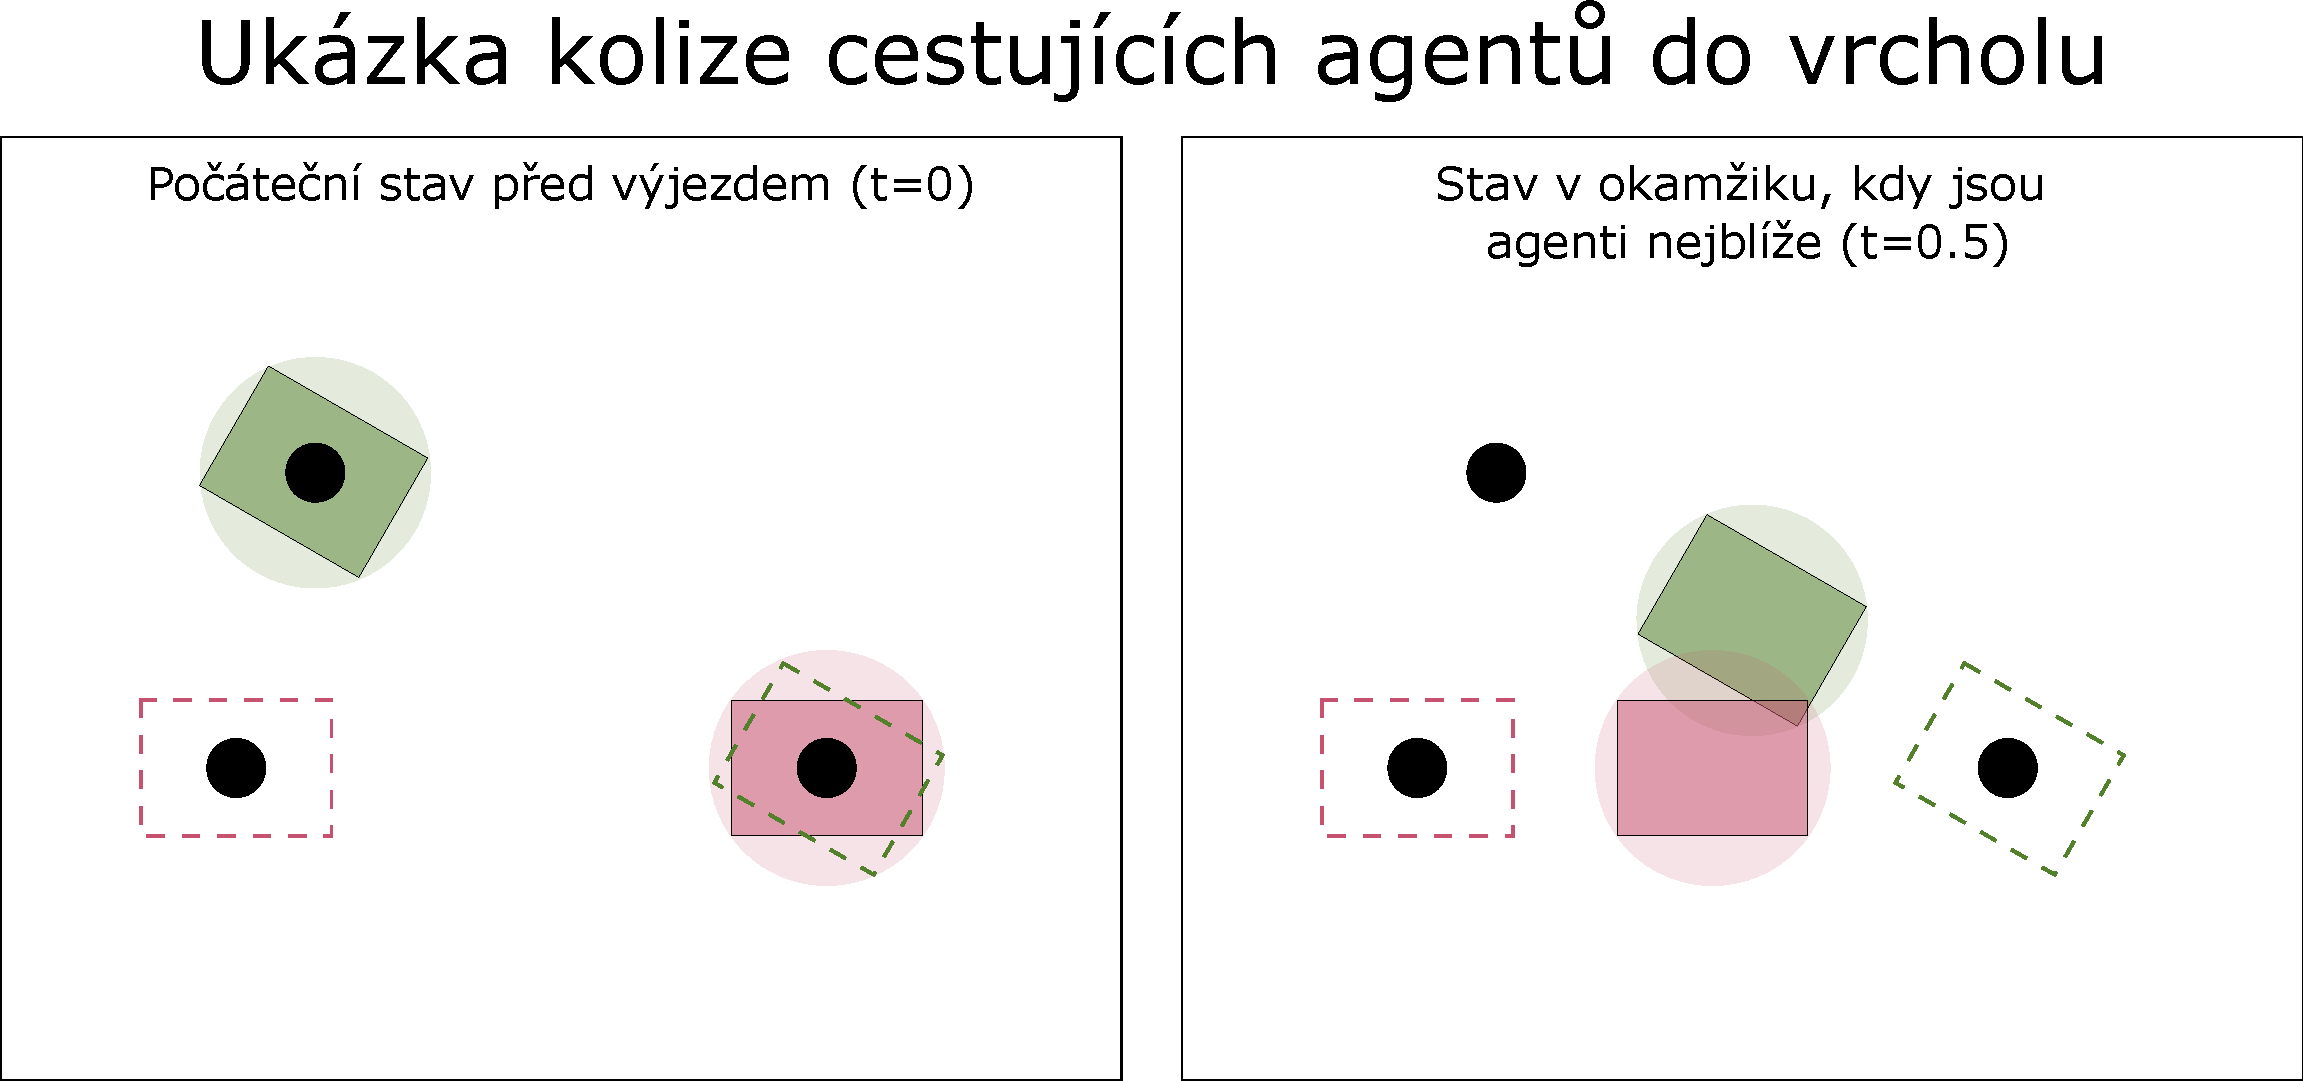
\includegraphics[width=\textwidth]{../img/kolize_cesta_z}
	\caption{
		Ukázka kolizní situace, která je detekována \hyperref[subsec:cesta_z_vrcholu]{kontrolou cesty z~vrcholu}.
		Na~obrázcích jsou černě zobrazeny vrcholy.
		Obdélníky reprezentují agenty a kruhy tvoří bezpečnou zónu příslušných agentů.
		Čárkované prázdné obdélníky značí cílové stavy agentů po~jednom kroku.
		Zelený agent je již naplánovaný, černevý je aktuálně plánován.
	}
	\label{fig:kolize_cesta_z}
\end{figure}

Formálně agent~$a$ cestuje z~$v$ do~$w$ v~kroku~$s$ a agent~$b$ cestuje z~$u$ do~$v$ opět v~kroku~$s$.
Pokud se na~situaci podívám z~pohledu druhého agenta (prohodím agenta $a$ za $b$), dostanu předchozí případ.
Z~tohoto důvodu můžu pro~kontrolu opět použít funkci \ref{str:safe_neighbour}, akorát prohodím parametry.
Výsledný algoritmus je následovný.

\labeltext{\textrm{safe\_step\_from}}{alg:kol_safe_step_from}
% @formatter:off
\begin{code}[fontsize=\footnotesize]
// konstanty tabulka obsazených pozic t

// agent a s poloměrem da cestuje z vrcholu v do w v kroku s
safe_step_from(s, v, w, da)
  b <- t[s + 1][v]
  if b is NULL
    return true

  u <- b.path[s]
  db <- diameter(b)
  return safe_neighbour(v, u, w, db, da)
\end{code}
% @formatter:on
